% =====================================================================
% NeuralFabric -- IEEE double-column manuscript (IEEEtran conference)
% Figures are read from paper_assets/ (generated by tools/make_paper_assets.py).
% Values in \chk{...} must be cross-checked against paper_assets/KEY_NUMBERS.md;
% values in \tbd{...} must be filled from paper_assets/tables.tex / KEY_NUMBERS.md.
% Before submission: redefine \chk and \tbd to plain #1 (see below) and
% make sure no \tbd remains.
% =====================================================================
\documentclass[conference]{IEEEtran}
\usepackage{amsmath,amssymb,amsfonts}
\usepackage{cite}
\usepackage{booktabs}
\usepackage{multirow}
\usepackage{array}
\usepackage{graphicx}
\graphicspath{{./}{../}}
\usepackage{textcomp}
\usepackage{xcolor}
\usepackage{algorithm}
\usepackage{algorithmic}
\usepackage{tikz}
\usetikzlibrary{arrows.meta,positioning,fit,calc}
\usepackage{url}

% ---- review markers (set both to {#1} for the final version) ----
\newcommand{\chk}[1]{\textcolor{blue}{#1}}
\newcommand{\tbd}[1]{\textcolor{red}{[#1]}}

\makeatletter
\newcommand{\linebreakand}{%
  \end{@IEEEauthorhalign}
  \hfill\mbox{}\par
  \mbox{}\hfill\begin{@IEEEauthorhalign}
}
\makeatother

\begin{document}

\title{NeuralFabric: Capacity-Guarded Predictive Rerouting with Telemetry-Driven Congestion Forecasting for Datacenter Fabrics}

\author{
\IEEEauthorblockN{Divyank Seervi}
\IEEEauthorblockA{\textit{School of Computer Science and Engineering}\\
\textit{Vellore Institute of Technology}\\
Vellore, India\\
divyank.seervi2024@vitstudent.ac.in}
\and
\IEEEauthorblockN{Choppa Madhu Dhanush Teja}
\IEEEauthorblockA{\textit{School of Computer Science and Engineering}\\
\textit{Vellore Institute of Technology}\\
Vellore, India\\
choppa.madhu2024@vitstudent.ac.in}
\linebreakand
\IEEEauthorblockN{Krish}
\IEEEauthorblockA{\textit{School of Computer Science and Engineering}\\
\textit{Vellore Institute of Technology}\\
Vellore, India\\
krish2024@vitstudent.ac.in}
\and
\IEEEauthorblockN{Srishti Agarwal}
\IEEEauthorblockA{\textit{School of Computer Science and Engineering}\\
\textit{Vellore Institute of Technology}\\
Vellore, India\\
srishti.agarwal2024@vitstudent.ac.in}
\linebreakand
\IEEEauthorblockN{Ganesh Khekare}
\IEEEauthorblockA{\textit{School of Computer Science and Engineering}\\
\textit{Vellore Institute of Technology}\\
Vellore, India\\
\tbd{guide e-mail}}
}

\maketitle

% ---------------------------------------------------------------------
\begin{abstract}
Datacenter fabrics provide many equal-cost paths, yet hash-based multipath forwarding cannot avoid links that are about to become congested, while reactive rerouting acts only after queues have grown and tends to move many flows at once. This work examines whether short-horizon congestion forecasts can be converted into safe route changes. A full-duplex, packet-conserving simulator of a k=4 Fat-Tree fabric is used to generate in-band-telemetry-style link and switch features for six synthetic workload families. A spatio-temporal graph convolutional and long short-term memory forecaster predicts per-link congestion five milliseconds ahead, and a capacity-guarded controller admits a route change only when the candidate path lowers predicted risk, respects bounded path stretch, cooldown and per-tick budgets, and passes a sequential capacity-reservation check. The evaluation uses a stratified scenario split, three training seeds, ten traffic seeds per family, calibrated thresholds, onset-only metrics, ablations and a sensitivity sweep. Learned forecasters rank future congestion better than persistence (average precision 0.947 versus 0.880), but removing the graph layers causes no measurable loss, and congestion onsets remain hard to anticipate. Every guarded variant reduces fabric-link drops by about 20--25\%, matching aggressive rerouting with roughly one-tenth of the route changes and lowering tail delay below static hashing, and the gain of guarded routing driven by the current congestion score persists on unseen traffic seeds; however, model-free guarded routing performs as well as forecast-driven guarded routing. Capacity-aware admission of route changes, rather than predictor complexity, therefore emerges as the decisive factor.
\end{abstract}

\begin{IEEEkeywords}
Datacenter networks, predictive routing, congestion forecasting, admission control, in-band network telemetry, graph neural networks, load balancing, Fat-Tree topology
\end{IEEEkeywords}

% =====================================================================
\section{Introduction}
\label{sec:intro}

\subsection{Background}
Datacenter networks interconnect thousands of servers that run distributed storage, analytics and machine-learning workloads. Measurement studies of production datacenters show that traffic is application-dependent and bursty rather than a smooth aggregate stream \cite{benson2010network}. To provide high bisection bandwidth with commodity switches, modern fabrics are built as multi-rooted trees such as the Fat-Tree \cite{alfares2008}, and related designs such as PortLand, VL2, BCube and Jellyfish further show that topology and path diversity determine how much routing freedom a controller has \cite{mysore2009portland,greenberg2009vl2,guo2009bcube,singla2012jellyfish}.

The standard way to use this path diversity is Equal-Cost Multi-Path (ECMP) forwarding, which hashes each flow onto one of the shortest paths \cite{hopps2000}. ECMP is simple and stable, but it is oblivious to load: two large flows can be hashed onto the same link while parallel links remain idle.

\subsection{Motivation}
When a link becomes congested, its queue grows, packets are dropped or delayed, and transport protocols back off. Every millisecond of queue build-up therefore translates into lost throughput and higher tail latency for the applications sharing that link. If congestion on a link could be anticipated a few milliseconds before it materialises, flows could be moved to an alternative equal-cost path in advance. This idea, known as predictive or proactive routing, has become more plausible with the availability of fine-grained In-band Network Telemetry (INT) and fast learning-based predictors.

\subsection{Existing Approaches and Their Limitations}
Dynamic flow scheduling systems such as Hedera and DevoFlow move large flows using global visibility of the network state \cite{alfares2010hedera,curtis2011devoflow}, and centralised optimisers such as ElasticTree adapt the active fabric to demand \cite{heller2010elastictree}. Distributed congestion-aware load balancers such as CONGA, HULA, DRILL, Presto and LetFlow react to measured path or queue conditions at flow, flowlet or packet granularity \cite{alizadeh2014conga,katta2016hula,ghorbani2015drill,he2015presto,vanini2017letflow}. These systems are effective, but they are reactive by construction: they respond after congestion has already been observed.

In parallel, Machine Learning (ML) models for networking have advanced quickly. Graph Neural Networks (GNNs) such as RouteNet model the relationship between topology, routing and performance \cite{rusek2020routenet}, and spatio-temporal graph models forecast traffic in transportation and communication networks \cite{li2018dcrnn,yu2018stgcn,zhao2020tgcn}. However, an accurate forecast does not automatically yield a good routing policy. When a forecast flags a link as risky, an unconstrained controller tends to move every affected flow to the same next-best path, simply shifting the bottleneck and generating excessive route churn.

\subsection{Research Gap}
Two questions are frequently conflated in prediction-driven networking: whether a model can forecast congestion, and whether acting on that forecast improves system-level behaviour. Existing studies seldom evaluate the second question against strong, model-free baselines that use the same action mechanism, and they rarely report whether a spatial graph component adds value over purely temporal modelling. Without such ablations, routing gains may be attributed to the predictor when they are in fact produced by the action policy.

\subsection{Proposed Solution and Novelty}
This paper presents NeuralFabric, an experimental framework that couples a telemetry-driven congestion forecaster with a capacity-guarded rerouting controller. The controller admits a forecast-driven route change only when the candidate path reduces predicted risk, keeps path stretch bounded, respects per-flow cooldown and a per-tick change budget, and passes a capacity check in which accepted moves sequentially reserve headroom, so that simultaneous decisions cannot exhaust the same spare capacity. The novelty of the work lies not in any individual component but in (i) the combination of forecast-gated rerouting with sequential capacity reservation, and (ii) an evaluation design that isolates the contribution of the forecaster from that of the admission policy.

\subsection{Contributions}
The main contributions of this paper are as follows:
\begin{enumerate}
\item A full-duplex, causal, packet-conserving simulator of a k=4 Fat-Tree fabric with hash-based ECMP, explicit per-direction queues and attribution of packet drops to host links and fabric links.
\item A spatio-temporal Graph Convolutional Network (GCN) and Long Short-Term Memory (LSTM) forecaster of per-link congestion, evaluated against persistence, an LSTM-only model and logistic regression with calibrated probabilities, validation-tuned thresholds and onset-only metrics.
\item A capacity-guarded rerouting controller that converts per-link risk scores into bounded, capacity-checked route changes.
\item An ablation and sensitivity methodology, including guard-only baselines, held-out workload families, multiple training and traffic seeds and paired bootstrap confidence intervals, which separates forecast quality from routing benefit.
\end{enumerate}

\subsection{Paper Organisation}
Section~\ref{sec:lit} critically reviews related work and establishes the research gap. Section~\ref{sec:method} describes the simulator, dataset, forecasting models and guarded controller with their mathematical formulation. Section~\ref{sec:setup} reports the experimental setup and evaluation metrics. Section~\ref{sec:results} presents the results, ablations, sensitivity analysis and discussion. Section~\ref{sec:conclusion} concludes the paper and outlines future scope.

% =====================================================================
\section{Literature Review}
\label{sec:lit}

\subsection{Datacenter Topologies and Multipath Routing}
The Fat-Tree architecture showed that commodity switches arranged as a multi-rooted tree can deliver full bisection bandwidth \cite{alfares2008}. PortLand added a scalable, fault-tolerant layer-2 fabric, VL2 exposed uniform high capacity through Valiant load balancing over a Clos network, BCube proposed a server-centric modular design and Jellyfish studied random regular graphs as an alternative to hierarchical layouts \cite{mysore2009portland,greenberg2009vl2,guo2009bcube,singla2012jellyfish}. These works establish that path multiplicity is the resource a load balancer exploits. ECMP remains the default way of using it because it is stateless and deterministic \cite{hopps2000}, but hash collisions between long-lived flows are a well-known weakness that motivates load-aware alternatives.

\subsection{Flow Scheduling and Congestion-Aware Load Balancing}
Hedera schedules large flows centrally to improve aggregate throughput over ECMP, and DevoFlow analyses the control-plane cost of obtaining the flow visibility that such scheduling requires \cite{alfares2010hedera,curtis2011devoflow}. ElasticTree demonstrates demand-driven reconfiguration of the active network \cite{heller2010elastictree}. Among distributed schemes, CONGA uses in-network congestion feedback with flowlet switching \cite{alizadeh2014conga}, HULA implements telemetry-driven path selection in programmable data planes \cite{katta2016hula}, DRILL performs micro load balancing using local queue information \cite{ghorbani2015drill}, Presto balances load at the network edge while handling packet reordering \cite{he2015presto}, and LetFlow exploits flowlets for resilience under asymmetry \cite{vanini2017letflow}. Centralised arbitration in Fastpass and priority-based transport in pFabric show that path selection, scheduling and transport interact strongly \cite{perry2014fastpass,alizadeh2013pfabric}. The common limitation for the present problem is that all of these mechanisms react to observed state; none of them evaluates whether acting on a forecast of future link state is beneficial.

\subsection{Congestion Control and In-Band Telemetry}
Data Center TCP (DCTCP) uses Explicit Congestion Notification (ECN) to keep queues short \cite{alizadeh2010dctcp}. DCQCN extends ECN-based control to Remote Direct Memory Access (RDMA) deployments \cite{zhu2015dcqcn}, TIMELY uses round-trip time as a congestion signal \cite{mittal2015timely}, and HPCC uses precise in-band telemetry to obtain link load information for rate control \cite{li2019hpcc}. PINT reduces the overhead of in-band telemetry while preserving its usefulness for congestion control and path tracing \cite{benbasat2020pint}. These works motivate per-hop queue and utilisation measurements as forecasting inputs, but they act on sending rates rather than on path admission.

\subsection{Graph and Temporal Learning for Network Prediction}
Graph convolutional networks propagate information along graph edges \cite{kipf2017gcn}, LSTM networks capture temporal dependence in sequences \cite{hochreiter1997lstm}, and surveys categorise convolutional, recurrent and spatio-temporal graph models as distinct families \cite{wu2021gnnsurvey}. In traffic forecasting, DCRNN combines diffusion convolution with recurrent units \cite{li2018dcrnn}, STGCN combines graph and temporal convolutions \cite{yu2018stgcn}, Graph WaveNet learns adaptive spatial dependencies \cite{wu2019graphwavenet} and T-GCN couples graph convolution with gated recurrent units \cite{zhao2020tgcn}. A recent survey reviews deep learning specifically for network traffic prediction and highlights the difficulty of generalising across traffic conditions \cite{aouedi2025survey}. In network modelling, RouteNet and RouteNet-Fermi predict delay, jitter and loss from topology, routing and traffic \cite{rusek2020routenet,ferriol2023routenetfermi}, and RouteNet-TGNN extends this line to temporal forecasting in dynamic networks \cite{ahmad2026routenettgnn}. These models establish that graph-temporal forecasting is feasible, but they report prediction accuracy rather than the routing consequences of acting on predictions.

\subsection{Learning-Based Routing and Control}
Learning to Route studies deep reinforcement learning for traffic engineering and highlights how difficult it is to replace algorithmic routing logic with learned policies \cite{valadarsky2017learning}. A hybrid Generative Adversarial Network (GAN) and Recurrent Neural Network (RNN) model has been integrated with Software-Defined Networking (SDN) for traffic engineering and access control, using synthetic traffic generation to support dynamic resource allocation and routing decisions \cite{khekare2023ganrnn}. GraphCC combines graph learning with multi-agent reinforcement learning to tune ECN parameters in datacenters \cite{bernardez2025graphcc}, and NTP-INT uses traffic prediction to plan telemetry paths on high-load switches \cite{zhang2025ntpint}. For Artificial Intelligence (AI) clusters, Hopper performs congestion-aware path selection for RDMA traffic \cite{nosrati2025hopper}, and FLB shows that fine-grained load balancing interacts non-trivially with lossless flow control \cite{hu2025flb}.

\subsection{Comparative Summary}
Table~\ref{tab:litreview} compares representative studies in terms of method, data or setting, key finding, strength and limitation with respect to forecast-driven rerouting.

\begin{table*}[!t]
\centering
\caption{Critical comparison of representative related work with respect to forecast-driven rerouting.}
\label{tab:litreview}
\footnotesize
\renewcommand{\arraystretch}{1.12}
\begin{tabular}{>{\raggedright\arraybackslash}p{1.9cm} >{\raggedright\arraybackslash}p{2.5cm} >{\raggedright\arraybackslash}p{2.2cm} >{\raggedright\arraybackslash}p{3.2cm} >{\raggedright\arraybackslash}p{2.7cm} >{\raggedright\arraybackslash}p{3.1cm}}
\toprule
\textbf{Study} & \textbf{Method} & \textbf{Data / setting} & \textbf{Key finding} & \textbf{Strength} & \textbf{Limitation (for this problem)}\\
\midrule
ECMP \cite{hopps2000} & Per-flow hashing over equal-cost paths & Analytical / standard practice & Simple, stable multipath forwarding & Stateless, deployable everywhere & Load-oblivious; hash collisions persist\\
Hedera \cite{alfares2010hedera} & Central scheduling of large flows & Fat-Tree testbed and simulation & Higher aggregate throughput than static hashing & Global view of large flows & Reactive; control-loop cost\\
CONGA \cite{alizadeh2014conga} & Congestion feedback with flowlet switching & Hardware testbed & Better load balance than ECMP under asymmetry & In-network, line rate & Reacts to measured state only\\
HULA \cite{katta2016hula} & Telemetry probes in programmable data planes & Programmable-switch implementation & Scalable congestion-aware path choice & Uses telemetry, distributed & No forecasting or admission guard\\
HPCC \cite{li2019hpcc} & Rate control from in-band telemetry & Testbed and simulation & Precise link-load feedback for transport & Fine-grained telemetry & Acts on rates, not paths\\
RouteNet \cite{rusek2020routenet} & GNN performance model & Simulated topologies & Accurate delay/jitter estimates & Topology-aware learning & No routing action evaluated\\
T-GCN \cite{zhao2020tgcn} & Graph convolution with recurrent units & Road-traffic datasets & Spatio-temporal forecasting gains & Joint spatial-temporal model & Not network congestion; no control\\
GAN-RNN SDN \cite{khekare2023ganrnn} & Hybrid GAN and RNN in SDN & Synthetic SDN traffic & 99.4\% reported accuracy for access control & Integrates learning with traffic engineering & Accuracy-centric; no guard-only ablation\\
GraphCC \cite{bernardez2025graphcc} & Graph learning with multi-agent reinforcement learning & Datacenter simulation & Learned ECN tuning & Learning in the control loop & Controls ECN, not path admission\\
NTP-INT \cite{zhang2025ntpint} & Traffic prediction for telemetry planning & High-load switches & Prediction-driven telemetry paths & Prediction feeds control & Different control variable\\
Hopper \cite{nosrati2025hopper} & Congestion-aware path selection & AI-cluster RDMA simulation & Path switching for RDMA traffic & Addresses AI workloads & Not a forecast-vs-guard study\\
\bottomrule
\end{tabular}
\end{table*}

\subsection{Review Analysis and Research Gap}
Three observations emerge from the review. First, deployed load balancers are predominantly reactive and therefore act only after queues have formed. Second, learning-based network models are mostly evaluated on prediction metrics, so it remains unclear whether their forecasts improve routing once acted upon. Third, when learned forecasts drive routing, results are seldom compared with model-free baselines that share the same action mechanism, and the value of the spatial graph component is seldom isolated. Consequently, the following questions remain open: (i) does a telemetry-driven forecaster rank future link congestion better than persistence on unseen workloads; (ii) does the spatial graph component add value over temporal modelling; and (iii) does forecast-driven rerouting outperform the same capacity-guarded controller driven by model-free signals? NeuralFabric is designed to answer these questions under a controlled, reproducible setting.

% =====================================================================
\section{Methodology}
\label{sec:method}

\subsection{System Overview}
Fig.~\ref{fig:arch} shows the end-to-end framework. Traffic generators produce flows on a Fat-Tree fabric; the simulator advances packets causally; a telemetry collector converts each tick into switch and link features; a forecaster produces calibrated per-link congestion probabilities; and the capacity-guarded controller decides whether any flow should change path. Route changes affect future traffic, closing the loop.

\begin{figure}[!t]
\centering
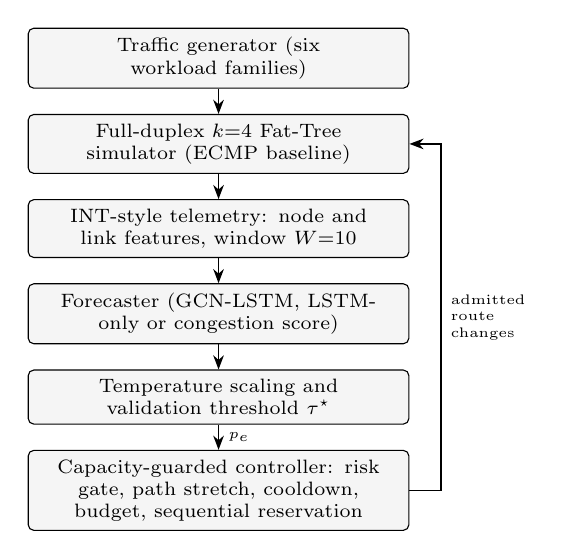
\begin{tikzpicture}[
  node distance=3.2mm,
  blk/.style={draw, rounded corners=2pt, align=center, font=\scriptsize, minimum height=6.5mm, text width=4.6cm, fill=gray!8},
  arr/.style={-{Stealth[length=1.8mm]}, semithick}]
\node[blk] (gen) {Traffic generator (six workload families)};
\node[blk, below=of gen] (sim) {Full-duplex $k{=}4$ Fat-Tree simulator (ECMP baseline)};
\node[blk, below=of sim] (tel) {INT-style telemetry: node and link features, window $W{=}10$};
\node[blk, below=of tel] (fc) {Forecaster (GCN-LSTM, LSTM-only or congestion score)};
\node[blk, below=of fc] (cal) {Temperature scaling and validation threshold $\tau^\star$};
\node[blk, below=of cal] (guard) {Capacity-guarded controller: risk gate, path stretch, cooldown, budget, sequential reservation};
\draw[arr] (gen) -- (sim);
\draw[arr] (sim) -- (tel);
\draw[arr] (tel) -- (fc);
\draw[arr] (fc) -- (cal);
\draw[arr] (cal) -- node[right, font=\tiny]{$p_e$} (guard);
\draw[arr] (guard.east) -- ++(4mm,0) |- node[pos=0.25, right, font=\tiny, align=left]{admitted\\route\\changes} (sim.east);
\end{tikzpicture}
\caption{NeuralFabric framework. Telemetry from the simulator feeds a per-link congestion forecaster whose calibrated probabilities $p_e$ drive a capacity-guarded rerouting controller; admitted route changes influence subsequent traffic.}
\label{fig:arch}
\end{figure}

\subsection{Network and Simulator Model}
The fabric is modelled as a graph $\mathcal{G}=(\mathcal{V},\mathcal{L})$ with switches and hosts as vertices and physical links as edges. A k=4 Fat-Tree contains 4 core, 8 aggregation and 8 edge switches, 16 hosts and 48 physical links, of which 32 interconnect switches \cite{alfares2008}. Each physical link $\{u,v\}$ is full-duplex and is represented by two directed links $(u,v)$ and $(v,u)$, each with capacity $C$ packets per tick and buffer $B$ packets. Time advances in ticks of 1~ms.

For a directed link $\ell$ at tick $t$, let $a_\ell(t)$ be arriving packets and $q_\ell(t)$ the queue occupancy. Accepted packets, drops, served packets and the queue update are
\begin{align}
\hat{a}_\ell(t) &= \min\{a_\ell(t),\, B - q_\ell(t)\}, \quad d_\ell(t)=a_\ell(t)-\hat{a}_\ell(t), \label{eq:accept}\\
s_\ell(t) &= \min\{q_\ell(t)+\hat{a}_\ell(t),\, C\}, \label{eq:serve}\\
q_\ell(t+1) &= q_\ell(t)+\hat{a}_\ell(t)-s_\ell(t). \label{eq:queue}
\end{align}
Packets advance at most one link per tick, so forwarding is causal. Over a run, the simulator asserts packet conservation,
\begin{equation}
P_{\text{offered}} = P_{\text{dropped}} + P_{\text{delivered}} + P_{\text{outstanding}},
\label{eq:conservation}
\end{equation}
and attributes every drop to a host link (a link with a host endpoint), a fabric link (switch-to-switch) or an unroutable flow, so that $D_{\text{total}}=D_{\text{host}}+D_{\text{fabric}}+D_{\text{unroutable}}$.

Baseline forwarding uses ECMP. For a flow $f$ from $s$ to $d$ with equal-cost shortest-path set $\Pi_{sd}$, the path index is
\begin{equation}
i_f = \mathrm{SHA256}(s \,\|\, d \,\|\, \mathrm{id}_f) \bmod |\Pi_{sd}|,
\label{eq:ecmp}
\end{equation}
which spreads flows across all core switches while keeping each flow on a single path.

\subsection{Dataset Generation}
No public dataset provides per-link, per-millisecond telemetry for a datacenter fabric together with the ability to replay routing decisions. A synthetic dataset was therefore generated with six traffic families, summarised in Table~\ref{tab:families}. Each scenario lasts $T=150$ ticks. Thirty scenarios (five per family, distinct random seeds) form the forecasting dataset, and a separate set of traffic seeds is used for routing evaluation.

\begin{table}[!t]
\centering
\caption{Synthetic traffic families used for data generation.}
\label{tab:families}
\footnotesize
\begin{tabular}{>{\raggedright\arraybackslash}p{1.7cm} >{\raggedright\arraybackslash}p{5.9cm}}
\toprule
\textbf{Family} & \textbf{Description}\\
\midrule
Uniform & Background flows between random host pairs at moderate rates\\
Hotspot & Incast: several sources send at high rate to one destination, plus background\\
Elephant/mice & Mixture of long, high-rate flows and short, low-rate flows\\
Stride & Pod-to-pod permutation that stresses the core layer\\
LLM-training & Large Language Model (LLM) training-inspired collective bursts (ring and all-to-all phases); not a trace replay\\
Mixed & Superposition of the above generators\\
\bottomrule
\end{tabular}
\end{table}

With a window of $W=10$ ticks and horizon $H=5$ ticks, each scenario yields $T-W-H+1=\chk{136}$ windows, each containing all 32 fabric links. The stratified split assigns three scenarios per family to training, one to validation and one to testing (18/6/6 scenarios, i.e.\ \chk{2,448/816/816} windows). Splitting by whole scenarios prevents overlapping windows from crossing partitions.

\subsection{Preprocessing and Feature Representation}
For each switch $v$, the node feature vector is
\begin{equation}
\mathbf{x}_v(t)=\Big[\tfrac{\bar{q}_v}{B},\, \tfrac{\sum s}{C\deg v},\, \min\!\big(1,\tfrac{\sum d}{C}\big),\, \tfrac{\sum q}{\sum B}\Big],
\label{eq:nodefeat}
\end{equation}
computed over the egress links of $v$ (average queue, throughput, drops and buffer usage). For each physical fabric link $e=\{u,v\}$, directional quantities are merged by taking the maximum over both directions, and the edge feature vector is
\begin{equation}
\mathbf{x}_e(t)=\big[\min(1,a/C),\;\; q/B,\;\; \min(1,d/C),\;\; s/C\big],
\label{eq:edgefeat}
\end{equation}
i.e.\ offered utilisation, normalised queue, normalised drops and served utilisation. All features lie in $[0,1]$. The features emulate per-hop in-band telemetry but are read directly from the simulator state.

The congestion score of link $e$ combines served load and queue build-up,
\begin{equation}
c_e(t)=\mathrm{clip}_{[0,1]}\!\left(\max\!\Big\{\frac{s_e(t)}{C},\; \tau_c\frac{q_e(t)}{\phi B}\Big\}\right),
\label{eq:score}
\end{equation}
with $\tau_c=0.85$ and $\phi=0.1$, and the binary label is $y_e(t)=\mathbb{1}[c_e(t)>\tau_c]$. A link is therefore labelled congested when it serves more than 85\% of capacity or holds more than 10\% of its buffer. The learning target for a window ending at tick $t$ is $y_e(t+H)$.

An \emph{onset} is a link-window for which $y_e(t)=0$ but $y_e(t+H)=1$; onsets are the cases where forecasting can add information beyond the current state.

\subsection{Forecasting Models}
\subsubsection{GCN-LSTM}
At each tick in the window, a two-layer GCN encodes node features \cite{kipf2017gcn}:
\begin{equation}
\mathbf{H}^{(l+1)}=\mathrm{ReLU}\!\left(\mathrm{LN}\big(\hat{\mathbf{D}}^{-1/2}\hat{\mathbf{A}}\hat{\mathbf{D}}^{-1/2}\mathbf{H}^{(l)}\mathbf{W}^{(l)}\big)\right),
\label{eq:gcn}
\end{equation}
where $\hat{\mathbf{A}}$ is the switch adjacency matrix with self-loops, $\hat{\mathbf{D}}$ its degree matrix, $\mathrm{LN}$ layer normalisation and $\mathbf{H}^{(0)}=\mathbf{X}(t)$. For link $e=\{u,v\}$ the per-tick input to the temporal model is
\begin{equation}
\mathbf{m}_e(t)=\mathbf{W}_p\big[\mathbf{h}_u(t)\,\|\,\mathbf{h}_v(t)\,\|\,\mathbf{x}_e(t)\big]+\mathbf{b}_p .
\label{eq:edgeemb}
\end{equation}
An LSTM \cite{hochreiter1997lstm} processes the sequence $\mathbf{m}_e(t-W+1),\dots,\mathbf{m}_e(t)$:
\begin{align}
[\mathbf{i}_t;\mathbf{f}_t;\mathbf{o}_t] &= \sigma(\mathbf{W}\mathbf{m}_t+\mathbf{U}\mathbf{h}_{t-1}+\mathbf{b}),\label{eq:lstm1}\\
\tilde{\mathbf{c}}_t &= \tanh(\mathbf{W}_c\mathbf{m}_t+\mathbf{U}_c\mathbf{h}_{t-1}+\mathbf{b}_c),\label{eq:lstm2}\\
\mathbf{c}_t &= \mathbf{f}_t\odot\mathbf{c}_{t-1}+\mathbf{i}_t\odot\tilde{\mathbf{c}}_t,\quad \mathbf{h}_t = \mathbf{o}_t\odot\tanh(\mathbf{c}_t).\label{eq:lstm3}
\end{align}
A two-layer perceptron maps the final hidden state to a logit $z_e$, and the calibrated probability is
\begin{equation}
p_e=\sigma\!\left(z_e/T_s\right),
\label{eq:temp}
\end{equation}
where $T_s$ is a temperature fitted on validation data \cite{guo2017calibration}. The GCN-LSTM has 17,985 trainable parameters.

\subsubsection{Baselines}
Four baselines use the same inputs and split. \emph{Binary persistence} predicts $\hat{y}_e(t+H)=y_e(t)$. \emph{Continuous persistence} uses the current score $c_e(t)$ of (\ref{eq:score}) as the prediction score. \emph{LSTM-only} removes the GCN and feeds the edge features $\mathbf{x}_e$ directly into the same LSTM and output head, which isolates the contribution of the spatial component. \emph{Logistic regression} fits one model per link on the flattened $W\times 4$ window.

\subsection{Training and Calibration}
Models are trained with weighted binary cross-entropy,
\begin{equation}
\mathcal{L}=-\frac{1}{N}\sum_{n}\big[w_+\, y_n\log p_n+(1-y_n)\log(1-p_n)\big],
\label{eq:loss}
\end{equation}
with positive-class weight $w_+=3$ to counter class imbalance. After training, the temperature is obtained by minimising the validation negative log-likelihood,
\begin{equation}
T_s^\star=\arg\min_{T_s>0}\; -\sum_{n\in\mathcal{V}}\log P\big(y_n \mid \sigma(z_n/T_s)\big),
\label{eq:tempfit}
\end{equation}
and the decision threshold is selected on validation data as
\begin{equation}
\tau^\star=\arg\max_{\tau}\; \mathrm{F1}\big(\{\mathbb{1}[p_n>\tau]\}_{n\in\mathcal{V}}\big).
\label{eq:thresh}
\end{equation}
Temperature scaling is monotonic, so ranking metrics are unchanged while probabilities become better calibrated.

\subsection{Capacity-Guarded Rerouting Controller}
Given calibrated link probabilities $p_e$, the risk of a path $\pi$ is
\begin{equation}
r(\pi)=\max_{e\in\pi} p_e .
\label{eq:risk}
\end{equation}
An active flow $f$ on path $\pi_f$ is considered only if $r(\pi_f)>\tau^\star$. Up to three candidate paths are generated as weighted simple paths with link cost $1+10\,p_e$. A candidate $\pi'$ is admissible only if all of the following hold:
\begin{align}
r(\pi_f)-r(\pi') &\ge \delta, \label{eq:improve}\\
|\pi'| &\le |\pi_f|+2, \label{eq:stretch}\\
D(e)+r_f+Q(e) &\le \alpha\, C(e)\quad \forall e\in \pi'\setminus\pi_f, \label{eq:capacity}
\end{align}
where $r_f$ is the flow rate, $D(e)$ the estimated demand on directed link $e$ (the larger of the summed active-flow rates and the observed arrivals), $Q(e)$ its queue and $\alpha$ the headroom factor. In addition, a flow may not be moved within $\kappa$ ticks of its previous move, at most $M$ moves are admitted per tick, and predictions older than one tick are rejected. Once a move is accepted, demand is reserved immediately:
\begin{equation}
D(e)\leftarrow D(e)-r_f\ \forall e\in\pi_f,\quad D(e)\leftarrow D(e)+r_f\ \forall e\in\pi',
\label{eq:reserve}
\end{equation}
so later decisions in the same tick cannot claim the same headroom. Flows are processed in decreasing order of current-path risk. Algorithm~\ref{alg:guard} summarises the procedure. The default parameters are $\delta=0.15$, $\alpha=0.90$, $\kappa=5$ and $M=4$.

\begin{algorithm}[!t]
\caption{Capacity-guarded rerouting (one tick)}
\label{alg:guard}
\footnotesize
\begin{algorithmic}[1]
\REQUIRE link probabilities $p$, threshold $\tau^\star$, active flows $F$, link states
\STATE Initialise demand $D(e)$ for every directed link; $n \leftarrow 0$
\FOR{$f \in F$ sorted by decreasing $r(\pi_f)$}
  \IF{$n \ge M$} \STATE \textbf{break} \ENDIF
  \IF{$r(\pi_f) \le \tau^\star$ \OR $f$ in cooldown} \STATE \textbf{continue} \ENDIF
  \FOR{$\pi'$ in up to 3 weighted simple paths of $f$}
    \IF{(\ref{eq:improve}), (\ref{eq:stretch}) and (\ref{eq:capacity}) hold}
      \STATE Reserve demand by (\ref{eq:reserve}); $\pi_f \leftarrow \pi'$; $n \leftarrow n+1$
      \STATE Start cooldown of $f$; \textbf{break}
    \ENDIF
  \ENDFOR
\ENDFOR
\end{algorithmic}
\end{algorithm}

The same controller is driven by different signals to form the routing strategies: forecaster probabilities (guarded GNN, guarded LSTM), the binary persistence label (guarded persistence) and the continuous score $c_e$ (guarded score). Reactive rerouting moves flows whose current path crosses a fabric link with utilisation above 0.9. Unguarded GNN rerouting moves flows away from links whose predicted probability exceeds a fixed alert threshold of 0.7; it keeps the five-tick per-flow cooldown but has no capacity check, per-tick budget, path-stretch bound or minimum-improvement condition.

\subsection{Evaluation Protocol}
Forecasting is evaluated on the held-out test scenarios only. Routing strategies are compared on identical traffic: for each family and traffic seed, every strategy receives exactly the same flows, which yields paired comparisons. Differences are summarised with paired bootstrap confidence intervals over (family, seed) pairs for routing and over test scenarios for forecasting.

% =====================================================================
\section{Experimental Setup}
\label{sec:setup}

\subsection{Environment}
All experiments were run on an HP 14s-dq2xxx laptop with an 11th-generation Intel Core i5-1135G7 processor (2.40~GHz, 4 cores, 8 logical processors), 8~GB Random-Access Memory (RAM) and Windows~11 Home (build 26200), using the Central Processing Unit (CPU) only (the integrated Intel Iris Xe graphics were not used). The software stack consists of Python~3.14, PyTorch~2.14.1 (CPU build), PyTorch Geometric~\chk{2.8}, NetworkX, NumPy and scikit-learn; inference timing uses two CPU threads.

\subsection{Hyperparameters and Training Procedure}
Table~\ref{tab:hyper} lists the hyperparameters. Training uses the Adam optimiser with learning rate $10^{-3}$, weight decay $10^{-4}$, batch size 32 and gradient clipping at 1.0, for at most 50 epochs with early stopping (patience 10) on validation average precision and learning-rate reduction on plateau (patience 5, factor 0.5). Each learned model is trained with three seeds; routing experiments with learned forecasters are repeated for all three seeds. Model selection, temperature fitting and threshold selection use the validation set only; the test scenarios and the routing traffic seeds are never used for any selection.

\begin{table}[!t]
\centering
\caption{Hyperparameters and experimental settings.}
\label{tab:hyper}
\footnotesize
\begin{tabular}{ll}
\toprule
\textbf{Setting} & \textbf{Value}\\
\midrule
Topology & k=4 Fat-Tree, 32 fabric links\\
Link capacity / buffer & 500 packets/tick / 2000 packets\\
Tick, scenario length & 1 ms, 150 ticks\\
Window $W$ / horizon $H$ & 10 / 5 ticks\\
GCN layers / hidden size & 2 / 64\\
LSTM layers / hidden size & 1 / 32\\
Dropout & 0.3\\
Optimiser & Adam, lr $10^{-3}$, weight decay $10^{-4}$\\
Batch size / max epochs & 32 / 50 (early stop, patience 10)\\
Positive-class weight $w_+$ & 3\\
Training seeds & 3\\
Guard: $\delta$, $\alpha$, $\kappa$, $M$ & 0.15, 0.90, 5 ticks, 4 moves/tick\\
Routing traffic seeds & 10 per family (3000--3009)\\
Sensitivity seeds & 10 per family (4000--4009)\\
\bottomrule
\end{tabular}
\end{table}

\subsection{Evaluation Metrics}
Congestion is a minority class (positive rate \chk{0.233} overall and \chk{0.035} among onset candidates), so accuracy alone would be misleading. With precision $P=\frac{TP}{TP+FP}$ and recall $R=\frac{TP}{TP+FN}$, the following metrics are reported:
\begin{align}
\mathrm{F1}&=\frac{2PR}{P+R}, \label{eq:f1}\\
\mathrm{AP}&=\sum_{k}(R_k-R_{k-1})\,P_k, \label{eq:ap}\\
\mathrm{Brier}&=\frac{1}{N}\sum_{n}(p_n-y_n)^2. \label{eq:brier}
\end{align}
Average precision (AP) summarises the precision--recall curve independently of the threshold and is the primary ranking metric; the area under the receiver operating characteristic curve (AUC) is also reported, and the Brier score measures calibration. All forecasting metrics are computed both overall and on onset windows. Routing performance is measured by total, fabric-link and host-link drops, delivered packets per tick, mean and 99th-percentile delivered delay, and route changes per run. The relative drop change with respect to ECMP is
\begin{equation}
\Delta_{\%}=100\cdot\frac{D_{\text{strategy}}-D_{\text{ECMP}}}{D_{\text{ECMP}}},
\label{eq:delta}
\end{equation}
and 95\% Confidence Intervals (CIs) are obtained with 2000 paired bootstrap resamples.

% =====================================================================
\section{Results and Discussion}
\label{sec:results}

\subsection{Forecast Quality}
Table~\ref{tab:forecast} and Fig.~\ref{fig:forecast} compare the forecasters on the test scenarios. Both learned temporal models rank future congestion clearly better than persistence: the GCN-LSTM reaches an AP of 0.947$\pm$0.003, compared with 0.880 for continuous persistence, a difference of +0.067 (95\% CI [+0.040, +0.131]). Calibration changed probabilities only marginally (fitted temperatures 0.79--0.98, Brier change at most 0.0016), indicating that the trained models were already close to calibrated.

\begin{table}[!t]
\centering
\caption{Forecast quality on test scenarios (mean $\pm$ std over three training seeds where applicable). The Brier score of continuous persistence is computed on the clipped congestion score, not on a probability.}
\label{tab:forecast}
\footnotesize
\setlength{\tabcolsep}{3.2pt}
\begin{tabular}{lccccc}
\toprule
\textbf{Predictor} & \textbf{F1} & \textbf{AP} & \textbf{AUC} & \textbf{Brier} & \textbf{Onset AP}\\
\midrule
GCN-LSTM & 0.893 & 0.947$\pm$0.003 & \chk{0.976} & 0.049 & \chk{0.184}\\
LSTM-only & 0.900 & \chk{0.946} & \chk{0.972} & 0.041 & \chk{0.192}\\
Logistic regression & \chk{0.865} & \chk{0.938} & \chk{0.968} & \chk{0.046} & \chk{0.180}\\
Persistence (cont.) & \chk{0.887} & 0.880 & \chk{0.961} & \chk{0.130} & \chk{0.163}\\
Persistence (binary) & \chk{0.887} & \chk{0.813} & \chk{0.926} & \chk{0.053} & \chk{0.035}\\
\bottomrule
\end{tabular}
\end{table}

\begin{figure}[!t]
\centering
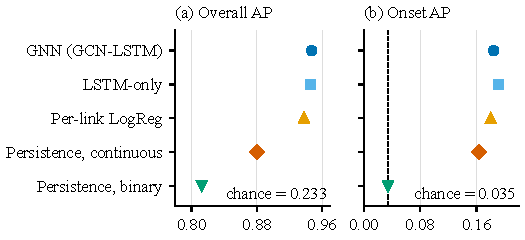
\includegraphics[width=\columnwidth]{paper_assets/fig_forecast.pdf}
\caption{Average precision overall (a) and on congestion onsets (b). Dashed lines mark the positive rate, i.e.\ the AP of a random predictor. Error bars show the standard deviation over three training seeds.}
\label{fig:forecast}
\end{figure}

Onsets remain difficult. All learned models obtain an onset AP of only about 0.18--0.19; the GCN-LSTM improves on continuous persistence by +0.021, with a confidence interval only just above zero. Most of the forecasting skill therefore lies in estimating the persistence and decay of existing congestion rather than in anticipating new congestion.

\subsection{Generalisation to Unseen Workload Families}
To test whether the models learn congestion dynamics rather than the generator, a pilot holdout experiment trained on five families and tested on the sixth, rotating through all six. In every rotation, the learned forecaster exceeded continuous persistence in AP with a confidence interval above zero, and the LSTM-only model remained within 0.009 AP of the GCN-LSTM. This pilot used 20 epochs and a single training seed, so it supports generalisation qualitatively rather than as a final estimate.

\subsection{Ablation Study}
Two ablations isolate the components of the framework.

\emph{Removing the spatial component.} The LSTM-only model matches the GCN-LSTM: the AP difference is +0.001 (95\% CI [$-0.003$, +0.014]), and LSTM-only has slightly better F1 (0.900 versus 0.893) and Brier score (0.041 versus 0.049). On a k=4 fabric with a 5~ms horizon, the future state of a link is determined mainly by the flows already on that link, and the switch-level node features are aggregates of the same link measurements that the temporal model already receives. Spatial message passing therefore adds no measurable information in this setting.

\emph{Removing the forecaster.} Replacing forecaster probabilities with model-free signals in the same guarded controller isolates the value of prediction for routing. Table~\ref{tab:routing} shows that guarded score, which uses only the current congestion score, achieves the largest total-drop reduction (5.72\%), followed by guarded LSTM (5.37\%), guarded GNN (5.27\%) and guarded persistence (4.86\%). None of the paired comparisons between guarded GNN and these alternatives is statistically significant (Table~\ref{tab:paired}); every confidence interval includes zero.

\begin{table*}[!t]
\centering
\caption{Routing outcomes per strategy over 6 families $\times$ 10 traffic seeds (model-based strategies averaged over three training seeds).}
\label{tab:routing}
\footnotesize
\setlength{\tabcolsep}{4pt}
\begin{tabular}{lccccccc}
\toprule
\textbf{Strategy} & \textbf{Total drops} & \textbf{Fabric drops} & \textbf{Host drops} & \textbf{Delivered} & \textbf{Mean delay} & \textbf{p99 delay} & \textbf{Reroutes}\\
 & \textbf{vs ECMP} & \textbf{vs ECMP} & \textbf{per run} & \textbf{pkt/tick} & \textbf{(ms)} & \textbf{(ms)} & \textbf{per run}\\
\midrule
ECMP & 0 (reference) & 0 (reference) & \chk{150,969} & \chk{2,508.2} & \chk{7.70} & \chk{15.47} & 0\\
Reactive & \chk{$-$4.15\%} & \chk{$-$17.05\%} & \chk{153,414} & \chk{2,561.9} & \chk{7.95} & \chk{17.60} & \chk{547.5}\\
Unguarded GNN & \chk{$-$5.51\%} & \chk{$-$26.46\%} & \chk{156,800} & \chk{2,587.8} & \chk{7.95} & \chk{17.17} & \chk{585.6}\\
Guarded GNN & $-$5.27\% & \chk{$-$22.98\%} & \chk{154,990} & \chk{2,587.6} & \chk{7.29} & \chk{14.04} & \chk{58.9}\\
Guarded LSTM & $-$5.37\% & \chk{$-$23.52\%} & \chk{155,128} & \chk{2,589.7} & \chk{7.30} & \chk{14.28} & \chk{47.8}\\
Guarded persistence & $-$4.86\% & \chk{$-$19.79\%} & \chk{153,718} & \chk{2,582.0} & \chk{7.28} & \chk{14.20} & \chk{47.8}\\
Guarded score & $-$5.72\% & \chk{$-$24.85\%} & \chk{155,259} & \chk{2,594.7} & \chk{7.26} & \chk{14.12} & \chk{37.9}\\
\bottomrule
\end{tabular}
\end{table*}

\begin{table}[!t]
\centering
\caption{Paired differences in total drops per run, guarded GNN minus alternative (95\% bootstrap CI).}
\label{tab:paired}
\footnotesize
\begin{tabular}{lcc}
\toprule
\textbf{Alternative} & \textbf{Mean difference} & \textbf{95\% CI}\\
\midrule
Guarded persistence & \chk{$-$889} & \chk{[$-$2,863, +878]}\\
Guarded score & \chk{+990} & \chk{[$-$463, +2,500]}\\
Guarded LSTM & \chk{+224} & \chk{[$-$751, +1,205]}\\
\bottomrule
\end{tabular}
\end{table}

\subsection{Routing Outcomes}
Fig.~\ref{fig:dropsplit} decomposes drops into fabric-link and host-link components. Every guarded variant reduces fabric-link drops by roughly 20--25\% relative to ECMP while performing few route changes. The total reduction is smaller (4.9--5.7\%) because part of the traffic that is no longer dropped in the fabric is subsequently dropped on the destination host link, which has no alternative path; rerouting cannot relieve an overloaded receiver.

Table~\ref{tab:routing} also exposes the cost of aggressive rerouting. Unguarded GNN rerouting reduces total drops by 5.51\%, more than three of the four guarded variants (only guarded score, at 5.72\%, is higher), and reactive rerouting by 4.15\%, but both perform more than 540 route changes per run and raise delivered delay above that of ECMP (99th percentile 17.17 and 17.60~ms versus 15.47~ms). The guarded variants obtain comparable drop reductions with 38--59 route changes per run and are the only strategies that lower delivered delay relative to ECMP (mean 7.26--7.30~ms versus 7.70~ms; 99th percentile 14.04--14.28~ms).

\begin{figure}[!t]
\centering
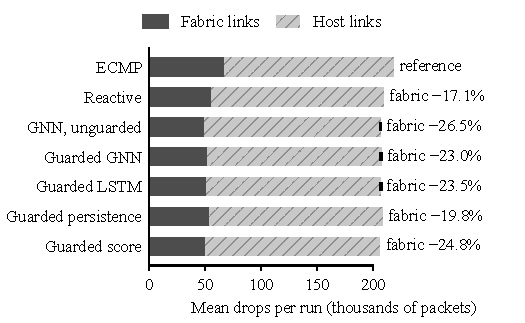
\includegraphics[width=\columnwidth]{paper_assets/fig_drops_split.pdf}
\caption{Mean drops per run split into fabric-link and host-link drops for each routing strategy; annotations give the fabric-drop change relative to ECMP.}
\label{fig:dropsplit}
\end{figure}

Fig.~\ref{fig:family} breaks the fabric-drop reduction down by workload family. The largest relative gain occurs for stride traffic, in which ECMP hashing places several pod-to-pod flows on the same core links. All ten stride traffic seeds generate the same set of sixteen flows (only rates and timing differ), so the stride result reflects a single collision pattern and should not be interpreted as ten independent confirmations. The LLM-training family produces no fabric-link drops under any strategy, as its bursts saturate host links. In the elephant/mice family, both reactive and unguarded GNN rerouting achieve fewer drops than any guarded variant, and in the mixed family unguarded GNN rerouting does so as well, in both cases at the cost of far more route changes (roughly 7--10 times as many in elephant/mice and 44--67 times as many in mixed).

\begin{figure}[!t]
\centering
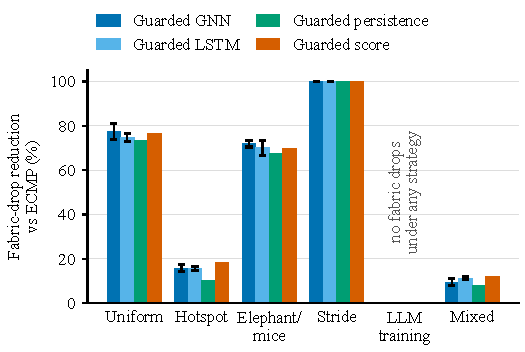
\includegraphics[width=\columnwidth]{paper_assets/fig_family.pdf}
\caption{Fabric-drop reduction relative to ECMP per traffic family for the guarded variants. The LLM-training family has no fabric drops under any strategy.}
\label{fig:family}
\end{figure}

\subsection{Sensitivity Analysis}
The per-tick change budget $M$ was varied for guarded score on ten new traffic seeds per family (4000--4009) that were not used anywhere else. Table~\ref{tab:sweep} shows that the gain over ECMP persists on unseen traffic, with a smaller magnitude than on the benchmark seeds ($-$4.28\% at the default $M=4$, with a paired confidence interval excluding zero). Raising $M$ to 8 or 16 changes the result by at most 0.51 percentage points in any family, so the change budget does not limit the controller; the weaker performance on elephant/mice and mixed traffic may instead stem from other guard parameters, such as the headroom factor or the minimum risk improvement, which were not varied in this study. Fig.~\ref{fig:tradeoff} places all strategies on a drops-versus-route-changes plane together with the sensitivity curve.

\begin{table}[!t]
\centering
\caption{Sensitivity of guarded score to the change budget $M$ on unseen traffic seeds 4000--4009.}
\label{tab:sweep}
\footnotesize
\begin{tabular}{ccc}
\toprule
\textbf{$M$ (moves/tick)} & \textbf{Total drops vs ECMP} & \textbf{Reroutes/run}\\
\midrule
2 & $-$3.70\% & 34.6\\
4 (default) & $-$4.28\% & 33.9\\
8 & $-$4.19\% & 32.9\\
16 & $-$4.19\% & 32.9\\
\bottomrule
\end{tabular}
\end{table}

\begin{figure}[!t]
\centering
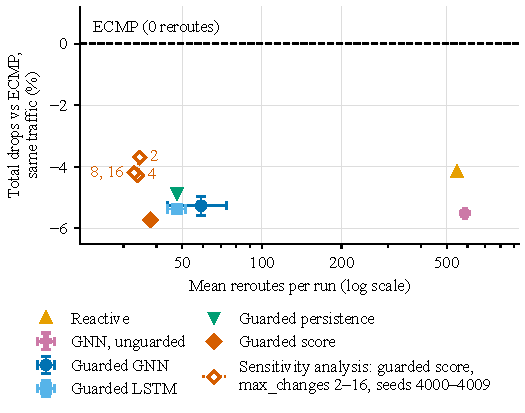
\includegraphics[width=\columnwidth]{paper_assets/fig_tradeoff.pdf}
\caption{Change in total drops relative to ECMP versus route changes per run (log scale). The curve shows the sensitivity analysis of guarded score over $M\in\{2,4,8,16\}$ on unseen traffic seeds.}
\label{fig:tradeoff}
\end{figure}

\subsection{Inference Latency}
Fig.~\ref{fig:inference} reports per-tick inference time. The GCN-LSTM has a median of 2.0~ms and a 99th percentile of 4.1~ms, and the LSTM-only model has a 99th percentile of 1.5~ms; only \chk{0.45\%} of GCN-LSTM calls exceed the 5~ms forecast horizon. These figures cover model inference only and exclude telemetry export, path computation and rule installation.

\begin{figure}[!t]
\centering
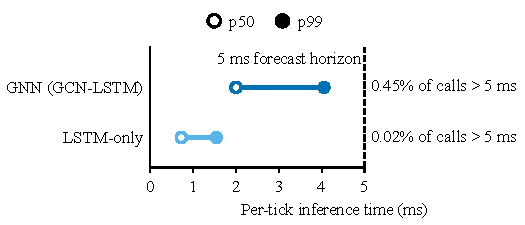
\includegraphics[width=\columnwidth]{paper_assets/fig_inference.pdf}
\caption{Median and 99th-percentile inference time per tick for the GCN-LSTM and LSTM-only forecasters relative to the 5~ms forecast horizon (CPU, two threads).}
\label{fig:inference}
\end{figure}

\subsection{Comparison with the State of the Art}
Production load balancers such as CONGA and HULA could not be re-implemented faithfully in the simulator, so the quantitative comparison uses reproducible baselines that represent the same design classes: static hashing (ECMP), reactive threshold rerouting, unguarded forecast-driven rerouting and model-free guarded rerouting. Qualitatively, NeuralFabric differs from the reactive systems in Table~\ref{tab:litreview} by acting on forecasts, and from learning-based models such as RouteNet and T-GCN by evaluating the routing consequences of predictions rather than prediction accuracy alone. Unlike accuracy-centric learning studies, the present evaluation reports guard-only ablations, onset metrics and paired confidence intervals, which expose where predictive skill does and does not translate into routing benefit.

\subsection{Discussion}
\emph{Key findings.} Learned temporal forecasters rank future link congestion better than persistence and generalise to unseen workload families, but the spatial GCN adds no measurable value on this topology, onsets remain hard to predict, and forecast-driven guarded routing does not outperform the same controller driven by the current congestion score. Guarded routing matches the drop reduction of aggressive rerouting with about one-tenth of the route changes and is the only approach that reduces delivered delay relative to ECMP.

\emph{Interpretation.} The guarded variants reduce drops more than reactive rerouting and less than unguarded GNN rerouting (the only exception is guarded score on total drops), but they do so with an order of magnitude fewer route changes and with lower delay. Because a 5~ms horizon is short relative to flow lifetimes, the current congestion score already carries most of the information needed to choose which flows to move, and the guard's admission rules, which include sequential capacity reservation, are consistent with avoiding the herd effect that affects unguarded rerouting, although the contribution of each rule was not isolated.

\emph{Implications.} For practitioners, investing in safe admission of route changes yields more benefit than investing in predictor complexity at short horizons. For researchers, forecast-driven routing should be evaluated against model-free baselines that share the same action mechanism; otherwise routing gains may be misattributed to prediction.

\emph{Limitations.} The simulator is a packet-batch model with 1~ms ticks and does not model transport congestion control, ECN, Priority-based Flow Control (PFC), RDMA ordering or rule-installation delay; telemetry is idealised; traffic is synthetic and the LLM-training family is collective-inspired rather than trace-driven; only a k=4 topology is studied; the forecasting test set contains six scenarios; and the holdout experiment is a single-seed pilot.

\emph{Recommendations.} Spatial graph models should be re-examined on larger fabrics, at longer horizons and with mechanisms that propagate congestion between links, where neighbour information is more likely to matter. Onset-focused objectives and calibrated uncertainty should be investigated if forecasts are to add value beyond current-state signals, and guard parameters should be tuned per workload, with each admission rule ablated individually.

% =====================================================================
\section{Conclusion and Future Scope}
\label{sec:conclusion}
This paper presented NeuralFabric, a framework that couples telemetry-driven congestion forecasting with a capacity-guarded rerouting controller in a full-duplex Fat-Tree simulator, and evaluated it with ablations that separate forecast quality from routing benefit. Learned temporal forecasters ranked future congestion clearly better than persistence and generalised to unseen workload families, whereas the spatial graph component and forecast-driven routing provided no measurable advantage over simpler alternatives. All guarded variants reduced fabric-link drops by about 20--25\%, matched the drop reduction of aggressive rerouting with roughly one-tenth of the route changes, lowered delivered delay below that of static hashing; the guarded variant driven by the current congestion score also retained its benefit on unseen traffic. The principal conclusion is that capacity-aware, sequentially reserved admission of route changes is the decisive factor for safe predictive rerouting at millisecond horizons.

Future work will evaluate the framework on larger topologies and longer horizons, introduce realistic flow-size distributions and packet-level simulation with transport and lossless flow control, study onset-oriented training objectives, tune guard parameters per workload, and investigate deployment on programmable data planes with measured control-loop latency.

% =====================================================================
\section*{Data and Code Availability}
The simulator, training and evaluation code, trained checkpoints, benchmark results and figure-generation scripts are available from the authors on reasonable request \tbd{or: at <repository URL>}. All datasets were generated synthetically with fixed random seeds and can be regenerated from the provided scripts.

% =====================================================================
\begin{thebibliography}{99}

\bibitem{benson2010network}
T.~Benson, A.~Akella, and D.~A.~Maltz, ``Network traffic characteristics of data centers in the wild,'' in \emph{Proc. 10th ACM Internet Measurement Conf. (IMC)}, 2010, pp.~267--280.

\bibitem{alfares2008}
M.~Al-Fares, A.~Loukissas, and A.~Vahdat, ``A scalable, commodity data center network architecture,'' in \emph{Proc. ACM SIGCOMM}, 2008, pp.~63--74, doi: 10.1145/1402958.1402967.

\bibitem{mysore2009portland}
R.~N.~Mysore, A.~Pamboris, N.~Farrington, N.~Huang, P.~Miri, S.~Radhakrishnan, V.~Subramanya, and A.~Vahdat, ``PortLand: A scalable fault-tolerant layer 2 data center network fabric,'' in \emph{Proc. ACM SIGCOMM}, 2009, pp.~39--50, doi: 10.1145/1594977.1592575.

\bibitem{greenberg2009vl2}
A.~Greenberg \emph{et al.}, ``VL2: A scalable and flexible data center network,'' in \emph{Proc. ACM SIGCOMM}, 2009, pp.~51--62, doi: 10.1145/1594977.1592576.

\bibitem{guo2009bcube}
C.~Guo \emph{et al.}, ``BCube: A high performance, server-centric network architecture for modular data centers,'' in \emph{Proc. ACM SIGCOMM}, 2009, pp.~63--74, doi: 10.1145/1594977.1592577.

\bibitem{singla2012jellyfish}
A.~Singla, C.-Y.~Hong, L.~Popa, and P.~B.~Godfrey, ``Jellyfish: Networking data centers randomly,'' in \emph{Proc. 9th USENIX Symp. Networked Systems Design and Implementation (NSDI)}, 2012, pp.~225--238.

\bibitem{hopps2000}
C.~Hopps, ``Analysis of an equal-cost multi-path algorithm,'' RFC~2992, IETF, Nov. 2000.

\bibitem{alfares2010hedera}
M.~Al-Fares, S.~Radhakrishnan, B.~Raghavan, N.~Huang, and A.~Vahdat, ``Hedera: Dynamic flow scheduling for data center networks,'' in \emph{Proc. 7th USENIX NSDI}, 2010, pp.~281--296.

\bibitem{curtis2011devoflow}
A.~R.~Curtis, J.~C.~Mogul, J.~Tourrilhes, P.~Yalagandula, P.~Sharma, and S.~Banerjee, ``DevoFlow: Scaling flow management for high-performance networks,'' in \emph{Proc. ACM SIGCOMM}, 2011, pp.~254--265.

\bibitem{heller2010elastictree}
B.~Heller, S.~Seetharaman, P.~Mahadevan, Y.~Yiakoumis, P.~Sharma, S.~Banerjee, and N.~McKeown, ``ElasticTree: Saving energy in data center networks,'' in \emph{Proc. 7th USENIX NSDI}, 2010.

\bibitem{alizadeh2014conga}
M.~Alizadeh \emph{et al.}, ``CONGA: Distributed congestion-aware load balancing for datacenters,'' in \emph{Proc. ACM SIGCOMM}, 2014, pp.~503--514, doi: 10.1145/2619239.2626316.

\bibitem{katta2016hula}
N.~Katta, M.~Hira, C.~Kompella, A.~Vahdat, and J.~Rexford, ``HULA: Scalable load balancing using programmable data planes,'' in \emph{Proc. ACM Symp. SDN Research (SOSR)}, 2016, doi: 10.1145/2890955.2890968.

\bibitem{ghorbani2015drill}
S.~Ghorbani, B.~Godfrey, Y.~Ganjali, and A.~Firoozshahian, ``Micro load balancing in data centers with DRILL,'' in \emph{Proc. 14th ACM Workshop on Hot Topics in Networks (HotNets)}, 2015, doi: 10.1145/2834050.2834107.

\bibitem{he2015presto}
K.~He, E.~Rozner, K.~Agarwal, W.~Felter, J.~Carter, and A.~Akella, ``Presto: Edge-based load balancing for fast datacenter networks,'' in \emph{Proc. ACM SIGCOMM}, 2015.

\bibitem{vanini2017letflow}
E.~Vanini, R.~Pan, M.~Alizadeh, P.~Taheri, and T.~Edsall, ``Let it flow: Resilient asymmetric load balancing with flowlet switching,'' in \emph{Proc. 14th USENIX NSDI}, 2017, pp.~407--420.

\bibitem{rusek2020routenet}
K.~Rusek, J.~Su{\'a}rez-Varela, P.~Almasan, P.~Barlet-Ros, and A.~Cabellos-Aparicio, ``RouteNet: Leveraging graph neural networks for network modeling and optimization in software-defined networks,'' \emph{IEEE J. Sel. Areas Commun.}, vol.~38, no.~10, pp.~2260--2270, 2020.

\bibitem{li2018dcrnn}
Y.~Li, R.~Yu, C.~Shahabi, and Y.~Liu, ``Diffusion convolutional recurrent neural network: Data-driven traffic forecasting,'' in \emph{Proc. Int. Conf. Learning Representations (ICLR)}, 2018.

\bibitem{yu2018stgcn}
B.~Yu, H.~Yin, and Z.~Zhu, ``Spatio-temporal graph convolutional networks: A deep learning framework for traffic forecasting,'' in \emph{Proc. 27th Int. Joint Conf. Artificial Intelligence (IJCAI)}, 2018, pp.~3634--3640, doi: 10.24963/ijcai.2018/505.

\bibitem{zhao2020tgcn}
L.~Zhao, Y.~Song, C.~Zhang, Y.~Liu, P.~Wang, T.~Lin, M.~Deng, and H.~Li, ``T-GCN: A temporal graph convolutional network for traffic prediction,'' \emph{IEEE Trans. Intell. Transp. Syst.}, vol.~21, no.~9, pp.~3848--3858, 2020, doi: 10.1109/TITS.2019.2935152.

\bibitem{perry2014fastpass}
J.~Perry, A.~Ousterhout, H.~Balakrishnan, D.~Shah, and H.~Fugal, ``Fastpass: A centralized zero-queue datacenter network,'' in \emph{Proc. ACM SIGCOMM}, 2014, pp.~307--318, doi: 10.1145/2619239.2626309.

\bibitem{alizadeh2013pfabric}
M.~Alizadeh \emph{et al.}, ``pFabric: Minimal near-optimal datacenter transport,'' in \emph{Proc. ACM SIGCOMM}, 2013, pp.~435--446, doi: 10.1145/2486001.2486031.

\bibitem{alizadeh2010dctcp}
M.~Alizadeh, A.~Greenberg, D.~A.~Maltz, J.~Padhye, P.~Patel, B.~Prabhakar, S.~Sengupta, and M.~Sridharan, ``Data center TCP (DCTCP),'' \emph{ACM SIGCOMM Comput. Commun. Rev.}, vol.~40, no.~4, pp.~63--74, 2010, doi: 10.1145/1851182.1851192.

\bibitem{zhu2015dcqcn}
Y.~Zhu \emph{et al.}, ``Congestion control for large-scale RDMA deployments,'' in \emph{Proc. ACM SIGCOMM}, 2015, pp.~523--536, doi: 10.1145/2785956.2787484.

\bibitem{mittal2015timely}
R.~Mittal \emph{et al.}, ``TIMELY: RTT-based congestion control for the datacenter,'' in \emph{Proc. ACM SIGCOMM}, 2015, pp.~537--550, doi: 10.1145/2829988.2787510.

\bibitem{li2019hpcc}
Y.~Li \emph{et al.}, ``HPCC: High precision congestion control,'' in \emph{Proc. ACM SIGCOMM}, 2019, pp.~44--58, doi: 10.1145/3341302.3342085.

\bibitem{benbasat2020pint}
R.~Ben~Basat, S.~Ramanathan, Y.~Li, G.~Antichi, M.~Yu, and M.~Mitzenmacher, ``PINT: Probabilistic in-band network telemetry,'' in \emph{Proc. ACM SIGCOMM}, 2020.

\bibitem{kipf2017gcn}
T.~N.~Kipf and M.~Welling, ``Semi-supervised classification with graph convolutional networks,'' in \emph{Proc. Int. Conf. Learning Representations (ICLR)}, 2017.

\bibitem{hochreiter1997lstm}
S.~Hochreiter and J.~Schmidhuber, ``Long short-term memory,'' \emph{Neural Computation}, vol.~9, no.~8, pp.~1735--1780, 1997, doi: 10.1162/neco.1997.9.8.1735.

\bibitem{wu2021gnnsurvey}
Z.~Wu, S.~Pan, F.~Chen, G.~Long, C.~Zhang, and P.~S.~Yu, ``A comprehensive survey on graph neural networks,'' \emph{IEEE Trans. Neural Netw. Learn. Syst.}, vol.~32, no.~1, pp.~4--24, 2021, doi: 10.1109/TNNLS.2020.2978386.

\bibitem{wu2019graphwavenet}
Z.~Wu, S.~Pan, G.~Long, J.~Jiang, and C.~Zhang, ``Graph WaveNet for deep spatial-temporal graph modeling,'' in \emph{Proc. 28th IJCAI}, 2019, pp.~1907--1913, doi: 10.24963/ijcai.2019/264.

\bibitem{aouedi2025survey}
O.~Aouedi, V.~A.~Le, K.~Piamrat, and Y.~Ji, ``Deep learning on network traffic prediction: Recent advances, analysis, and future directions,'' \emph{ACM Comput. Surv.}, vol.~57, no.~6, pp.~1--37, 2025, doi: 10.1145/3703447.

\bibitem{ferriol2023routenetfermi}
M.~Ferriol-Galm{\'e}s \emph{et al.}, ``RouteNet-Fermi: Network modeling with graph neural networks,'' \emph{IEEE/ACM Trans. Netw.}, vol.~31, no.~6, pp.~3080--3095, 2023, doi: 10.1109/TNET.2023.3269983.

\bibitem{ahmad2026routenettgnn}
S.~Ahmad, G.~S.~Rao, H.~A.~M.~Abdeljaber, E.~S.~N.~Joshua, F.~A.~Abdalla, and H.~Gadi, ``RouteNet-TGNN: A temporal graph neural network for delay and loss forecasting in dynamic communication networks,'' \emph{J. Commun.}, vol.~21, no.~2, pp.~211--225, 2026, doi: 10.12720/jcm.21.2.211-225.

\bibitem{valadarsky2017learning}
A.~Valadarsky, M.~Schapira, D.~Shahaf, and A.~Tamar, ``Learning to route,'' in \emph{Proc. 16th ACM Workshop on Hot Topics in Networks (HotNets)}, 2017, pp.~185--191, doi: 10.1145/3152434.3152441.

\bibitem{khekare2023ganrnn}
G.~Khekare, K.~P.~Kumar, K.~N.~Prasanthi, S.~R.~Godla, V.~Rachapudi, M.~S.~A.~Ansari, and Y.~A.~B.~El-Ebiary, ``Optimizing network security and performance through the integration of hybrid GAN-RNN models in SDN-based access control and traffic engineering,'' \emph{Int. J. Adv. Comput. Sci. Appl. (IJACSA)}, vol.~14, no.~12, 2023, doi: 10.14569/IJACSA.2023.0141262.

\bibitem{bernardez2025graphcc}
G.~Bern{\'a}rdez, J.~Su{\'a}rez-Varela, X.~Shi, S.~Xiao, X.~Cheng, P.~Barlet-Ros, and A.~Cabellos-Aparicio, ``GraphCC: A practical graph learning-based approach to congestion control in datacenters,'' \emph{Comput. Netw.}, vol.~257, art.~110981, 2025, doi: 10.1016/j.comnet.2024.110981.

\bibitem{zhang2025ntpint}
P.~Zhang, H.~Zhang, Y.~Dai, C.~Zeng, J.~Wang, and J.~Liao, ``NTP-INT: Network traffic prediction-driven in-band network telemetry for high-load switches,'' \emph{J. Netw. Comput. Appl.}, vol.~242, art.~104265, 2025, doi: 10.1016/j.jnca.2025.104265.

\bibitem{nosrati2025hopper}
E.~Nosrati and M.~Ghaderi, ``Congestion-aware path selection for load balancing in AI clusters,'' arXiv:2506.08132, 2025.

\bibitem{hu2025flb}
J.~Hu, W.~Li, X.~Liu, J.~Wang, B.~Liu, P.~Yin, J.~Wang, J.~Huang, and K.~Chen, ``FLB: Fine-grained load balancing for lossless datacenter networks,'' in \emph{Proc. USENIX Annu. Tech. Conf. (ATC)}, 2025.

\bibitem{guo2017calibration}
C.~Guo, G.~Pleiss, Y.~Sun, and K.~Q.~Weinberger, ``On calibration of modern neural networks,'' in \emph{Proc. 34th Int. Conf. Machine Learning (ICML)}, PMLR vol.~70, 2017, pp.~1321--1330.

\end{thebibliography}

\end{document}
